% Copyright (c) 2021-10-07 Eclipse Arrowhead Project
%
% This program and the accompanying materials are made available under the
% terms of the Eclipse Public License 2.0 which is available at
% http://www.eclipse.org/legal/epl-2.0.
%
% SPDX-License-Identifier: EPL-2.0

We, the Eclipse Arrowhead project, here present and authoritative set of Arrowhead concept definitions, meant to serve as the foundational language for discussions about and the modeling of Arrowhead-based designs.
This document exists to help mitigate compatibility and consistency issues in software, tooling, models, documentation and all other things of relevance to the Arrowhead framework.

\subsection{The Arrowhead Framework and Industry 4.0}
\label{sec:introduction:arrowhead}

The Arrowhead framework is two things.
Firstly, it is a set of assumptions, concepts, values and practices that frame the problem domain of \textit{designing service-oriented Industry 4.0 systems}.
Secondly, it is a set of software specifications, implementations and other artifacts meant to help address that problem domain.
As have already been established, this document is concerned primarily with essential concepts of the Arrowhead framework.

What is Industry 4.0 and how does Arrowhead relate to it?
We understand Industry 4.0 to be the expectation that factory automation will keep becoming increasingly computerized, digitized and interconnected.
More aspects of and surrounding manufacturing is handled by computers, more information is being made available to computers and, finally, comparatively more computers are given the opportunity to collect, communicate and act on that information.
This development is leading to increased industrial efficiency and flexibility, as machines become able to perform more of the work traditionally assigned to humans.
However, it also leads to new magnitudes of complexity, something currently prevailing automation systems are unable to manage.

The Arrowhead framework is a means to address this explosion of industrial complexity.
It provides a foundation for service-oriented communication between Industry 4.0 systems, such that interoperability, security, safety and other major concerns can be addressed efficiently and effectively.
It allows for system capabilities to be described, shared and exploited dynamically by communicating machines.

\subsection{Scope}
\label{sec:introduction:scope}

In this document, we outline a \GlossaryHyperRef{model-reference}{\textit{reference model}}.
We understand such to be a set of definitions for technical concepts of fundamental importance to a specific problem domain.
Such a document does not specify how its definitions should be used to design systems, either abstract or concrete.
Neither does it build upon or endorse any particular modeling tools or languages.

Reference models can be used as vocabularies for defining \GlossaryHyperRef{architecture-reference}{reference architectures}, which in turn can be used to derive \GlossaryHyperRef{architecture}{concrete architectures} and, finally, \GlossaryHyperRef{implementation-software}{software implementations}, as illustrated in Figure \ref{fig:reference-model}.

\vspace*{\fill}

\begin{figure}[ht]
  \centering
  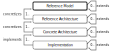
\includegraphics{figures/reference-model}
  \caption{
    The steps from reference model to implementation, going from highly abstract to entirely concrete.
    Reference models define fundamental concepts, reference architectures add abstract design constraints, concrete architectures makes those limits practically realizable, while implementations represent their actual realization.
  }
  \label{fig:reference-model}
\end{figure}

\vspace*{\fill}

\newpage

\subsection{Primary Audiences}
\label{sec:introduction:audiences}

This document is being written and maintained with the following primary audiences in mind:

\begin{itemize}
\item \textit{System architects, integrators and developers} designing, integrating or developing Arrowhead systems.
\item \textit{Standardization engineers and researchers} seeking to extend, analyze or improve upon Arrowhead.
\item \textit{Decision makers, users and other stakeholders} that need to understand fundamental Arrowhead concepts.
\end{itemize}

Those seeking a less technically rigorous description of Arrowhead may want to focus their reading on Section \ref{sec:arrowhead}.
Others are advised to read all sections carefully, in the order they are presented, except for Section \ref{sec:glossary}.
That section contains a glossary of significant terms and abbreviations and is meant to be used as a reference for modeling and documentation efforts.
Some may, however, find it rewarding to read it from beginning to end.

\subsection{Notational Conventions}
\label{sec:introduction:conventions}

The following conventions regarding diagrams, references and requirements are adhered to throughout this document.
All three of them were selected by virtue of being deemed unsurprising to our primary audiences.

\subsubsection{Diagrams}

A box with a name inside it denotes a named \GlossaryHyperRef{entity}{entity}.
A named arrow between boxes denotes the \GlossaryHyperRef{relationship}{relationship} implied by the name.
If a named arrow has an associated positive integer or range, the relation is to be considered as extending to the number of distinct entities indicated by that integer or range.
A range is denoted by $x..y$, where $x$ and $y$ are positive integers and $x<y$.
Omitting $y$ when using the range notation (e.g. $1..$) means that the range is infinite from $x$.
A box with a dotted border represents a group.
The entities explicitly placed within the box may or may not represent all entities that belong to that group.
See Figure \ref{fig:reference-model} for an example of this graphical notation being used.

Note that this document does \textit{not} define an Arrowhead profile for SysML \cite{omg2019sysml}, or any other modeling language.
As we cover later in Section \ref{sec:conformance}, however, we do expect all models based on this document not to contradict any of its definitions.

\subsubsection{References}

Square brackets around numbers (e.g. \cite{delsing2017iot}) are references to the reference list in Section \ref{sec:references}.
The number within the brackets of any given reference corresponds to the entry with the same number in the reference list.

References within this document are hyperlinked, which means that those reading it electronically can click the references and immediately be taken to their targets.
Special treatment is given to references targeting Section \ref{sec:glossary}, the \nameref{sec:glossary}.
These are displayed as regular text rendered with blue color.

\subsubsection{Requirements}

Use of the words \textbf{must}, \textbf{must not}, \textbf{required}, \textbf{should}, \textbf{should not}, \textbf{recommended}, \textbf{may}, and \textbf{optional} are to be interpreted as follows when used in this document: \textbf{must} and \textbf{required} denote absolute requirements that must be adhered to for a described entity to be considered as compliant to this reference model; \textbf{must not} denotes an absolute prohibition; \textbf{should}, \textbf{should not} and \textbf{recommended} denote recommendations that should be deviated from only if special circumstances make it relevant; and, finally, \textbf{may} and \textbf{optional} denote something being truly optional.
These word definitions are derived from and are meant to capture what is outlined in RFC 2119 \cite{bradner1997keywords}.

These word definitions have particular bearing on Section \ref{sec:conformance}, which is concerned with what documents and models can be considered conformant to or compliant with this document.
They do, however, apply to all parts of the document.

\subsection{Relationships to Other Documents}
\label{sec:introduction:relationships}

The reference model outlined in this document is based primarily on the following works:

\begin{enumerate}
\item \textit{Reference Architecture Model Industrie 4.0} (RAMI4.0) \cite{adolphs2016reference}, which outlines an ontological and architectural view of Industry 4.0.
As RAMI4.0 is a reference \textit{architecture} rather than a reference \textit{model}, we have only been concerned with what concepts it defines and what problems it frames.
The recommendations it makes regarding how Industry 4.0 systems \textit{should} be designed have not been considered.
This delimitation excludes its ``architectural layers'', ``life-cycle \& value-stream'' phases and ``hierarchical levels'', as well as the abstract design of its ``asset administrative shell''.
These excluded aspects are neither condemned nor endorsed by this document.
They are simply outside its scope.

\item \textit{Reference Model for Service Oriented Architecture} (SOA-RM) \cite{mackenzie2006reference}, which provides a standardized definition of SOA.
While RAMI4.0 does not include SOA-RM in its reference list, it does mention the standard and requires that all communications adhere to SOA principles, which should mean that the two standards are mostly compatible.
Even though we have found their concept definitions may be slight different, we have not found any major discrepancies.

\item \textit{IoT Automation: Arrowhead Framework} (IoTA:AF) \cite{delsing2017iot}, which significantly includes an overview of the \textit{local automation cloud} concept in its second chapter, as well as the \textit{Arrowhead framework architecture} in its third chapter.
While the strictly architectural aspects of IoTA:AF are out of scope, the two chapters contain several definition with a high degree of relevance to this document.

\end{enumerate}

You are not assumed to have read any of the above documents prior to reading this.
Concepts derived from the above sources are reiterated in this document as necessary.
Only adherence to IoTA:AF is observed strictly, which means that concept definitions presented here may diverge from those of the other two works.
All significant name differences are noted in the glossary of Section \ref{sec:glossary} under each definition of concern.

\subsection{Section Overview}
\label{sec:introduction:sections}

The remaining sections of this document are organized as follows:
\vspace*{2mm}
\begin{itemize}[leftmargin=2cm,rightmargin=0pt,labelwidth=2cm,labelsep=0pt,itemindent=0pt,parsep=0.1cm,topsep=0.1cm,align=left]

\item[Section \ref{sec:introduction}]
This section.

\item[Section \ref{sec:arrowhead}]
An informal overview of Arrowhead, serving both to provide a workable summary of the framework and to prepare readers for better understanding Section \ref{sec:model}.

\item[Section \ref{sec:model}]
The formal and normative description of Arrowhead.
Each of its subsections is concerned with one major Arrowhead concept, ranging from entities to systems-of-local-clouds.

\item[Section \ref{sec:conformance}]
A brief list of requirements, meant to help determine whether or not a given model or document is conforming to this reference model.

\item[Section \ref{sec:glossary}]
Lists all significant terms and abbreviations presented in this document in alphabetical order.

\item[Section \ref{sec:references}]
Lists references to publications referred to in this document.

\item[Section \ref{sec:revision}]
Records the history of changes made to this document.

\end{itemize}
